% ***************************************************
% FORMATO.
% ***************************************************
\documentclass[a4paper,12pt]{article}
% Input encoding.
% Idioma.
\usepackage[spanish, es-tabla]{babel}
\usepackage[utf8]{inputenc}
% Ver pagina 92 de "The not so short introduction to Latex" por Tobias Oetiker
% para entender que hacen estos paquetes.
\usepackage{lmodern}
\usepackage[T1]{fontenc}
\usepackage{textcomp}
% Paquete para utilizar el font Times Roman de Adobe por defecto.
\usepackage{mathptmx}

%Manejo de márgenes
%Agrega 2cm al ancho por defecto (usado junto con hoffset, no se pierde el centrado)
\addtolength{\textwidth}{2cm}
%Quita 1cm al margen, pero mantiene la relación repecto de cada margen
\addtolength{\hoffset}{-1cm}
\addtolength{\textheight}{2cm}
\addtolength{\voffset}{-1cm}
\setlength{\headheight}{14pt}

% Paquete para manejo de headers y footers.
\usepackage{fancyhdr}
\usepackage{lastpage}
% Determinación del estilo de página (encabezado y pie). Debe ir luego del bloque de manejo de margenes para que
% no haya problemas de dimensiones. Por ejemplo, que el texto quede mas ancho que el encabezado o pie.
\pagestyle{fancy}
% Se borra el header y footer por defecto.
\fancyhf{}
\lhead{\small TP1 [1C2020]}
\chead{}
\rhead{\small [66.20] Organización de Computadoras}
\rfoot{}
\cfoot{Página {\thepage} de \pageref{LastPage}}
\lfoot{}

% Paquete para manejo de textos en varbatim en varios lugares del documento, por ejemplo en los headers.
\usepackage{fancyvrb}
% Paquete para manejo de boxes de manera mas flexible.
\usepackage{fancybox}

% Para no mostrar el numero de pagina, usar las siguientes dos lineas:
%\thispagestyle{empty}
%\setcounter{savepage}{\thepage}

% Paquete para hacer subrayados, poner textos en color y resaltar texto en color.
% Lo bueno de este paquete es que no tira errores de fullbox como cuando se usa \colorbox{declared-color}{text}.
% El unico problema es que no soporta acentos desde el teclado (tira un error de UTF8). Hay que incluirlos usando \'.
\usepackage{soul}
% Configura el paquete @SOUL para que el resaltado de texto sea rojo. La sintaxis es \hl{text}.
\sethlcolor{red}

% Paquete que deja sangria luego de comenzada una seccion nueva.
%\usepackage{indentfirst}

% Se define una macro para poner double quotes de manera simple. El uso es \quotes{Hello World!}.
\newcommand{\quotes}[1]{``#1''}

% ***************************************************
% MATEMATICA.
% ***************************************************
\usepackage{amsmath}
% Formato de numeracion de ecuaciones por seccion. Ej. seccion x, ecuacion y: (x.y)
\numberwithin{equation}{section}
\numberwithin{figure}{section}

% Simbolos matematicos. Por ej. la 'R' de reales, etc...
\usepackage{amssymb}
\usepackage{amsfonts}

\usepackage{mathtools}

% Paquete para arrays de ecuaciones.
\usepackage[retainorgcmds]{IEEEtrantools}
% Unidad imaginaria.
\newcommand{\iu}{{j\mkern1mu}}
% Contador de uso generico.
\newcounter{hipotesis_ct}
\setcounter{hipotesis_ct}{1}

% Operador 'derivada'.
\makeatletter
\providecommand*{\diff}%
{\@ifnextchar^{\DIfF}{\DIfF^{}}}
\def\DIfF^#1{%
	\mathop{\mathrm{\mathstrut d}}%
	\nolimits^{#1}\gobblespace}
\def\gobblespace{%
	\futurelet\diffarg\opspace}
\def\opspace{%
	\let\DiffSpace\!%
	\ifx\diffarg(%
	\let\DiffSpace\relax
	\else
	\ifx\diffarg[%
	\let\DiffSpace\relax
	\else
	\ifx\diffarg\{%
	\let\DiffSpace\relax
	\fi\fi\fi\DiffSpace}

% Uso:
% \pderiv[n]{A}{B}
\providecommand*{\deriv}[3][]{%
	\frac{\diff^{#1}#2}{\diff #3^{#1}}}
\providecommand*{\pderiv}[3][]{%
	\frac{\partial^{#1}#2}%
	{\partial #3^{#1}}}

% Operadores 'valor absoluto' y 'norma'.
% Uso: \abs{123} \norm{123} \abs*{123} \norm*{123}
\DeclarePairedDelimiter\abs{\lvert}{\rvert}%
\DeclarePairedDelimiter\norm{\lVert}{\rVert}%
% Swap the definition of \abs* and \norm*, so that \abs
% and \norm resizes the size of the brackets, and the 
% starred version does not.
\makeatletter
\let\oldabs\abs
\def\abs{\@ifstar{\oldabs}{\oldabs*}}
%
\let\oldnorm\norm
\def\norm{\@ifstar{\oldnorm}{\oldnorm*}}
\makeatother

% Operadores para escribir vectores en negrita directamente.
% Ej:  $\vecbf{v} = 5\vechat{k}$ 
\newcommand{\vecbf}[1]{\mathbf{#1}}
% Operador para escribir en negrita todo lo que tenga hat.
\newcommand{\vechat}[1]{\hat{\mathbf{#1}}}

% ***************************************************
% CODIGO FUENTE.
% ***************************************************
% Paquetes para pseudocodigo.	
\usepackage{lgrind}
\usepackage{algorithm}
\usepackage{algpseudocode}
\makeatletter
\renewcommand{\ALG@name}{Algoritmo}
\renewcommand{\listalgorithmname}{Lista de \ALG@name s}
\algrenewcommand\algorithmicensure{\textbf{Salida:}}
\algrenewcommand\algorithmicrequire{\textbf{Entrada:}}
\algnewcommand{\LineComment}[1]{\State \(\triangleright\) #1}
\makeatother

% Paquete para incluir codigo de MatLab.
\usepackage[numbered,framed]{matlab-prettifier}
% Paquete para control de colores. Ya lo carga 'matlab-prettifier'.
\PassOptionsToPackage{usenames,dvipsnames}{xcolor}

% Fuente: http://en.wikibooks.org/wiki/LaTeX/Colors
\definecolor{Apricot}{RGB}{253,199,130}
\definecolor{Aquamarine}{RGB}{0,181,202}
\definecolor{Bittersweet}{RGB}{192,79,23}
\definecolor{Black}{RGB}{0,0,0}
\definecolor{Blue}{RGB}{0,0,255}
\definecolor{BlueGreen}{RGB}{0,179,184}
\definecolor{BlueViolet}{RGB}{71,57,146}
\definecolor{BrickRed}{RGB}{182,50,28}
\definecolor{Brown}{RGB}{121,37,0}
\definecolor{BurntOrange}{RGB}{247,146,29}
\definecolor{CadetBlue}{RGB}{116,114,154}
\definecolor{CarnationPink}{RGB}{242,130,180}
\definecolor{Cerulean}{RGB}{0,162,227}
\definecolor{CornflowerBlue}{RGB}{65,176,228}
\definecolor{Cyan}{RGB}{0,174,239}
\definecolor{Dandelion}{RGB}{253,188,66}
\definecolor{DarkOrchid}{RGB}{164,83,138}
\definecolor{Emerald}{RGB}{0,169,157}
\definecolor{ForestGreen}{RGB}{0,155,85}
\definecolor{Fuchsia}{RGB}{140,54,140}
\definecolor{Goldenrod}{RGB}{255,223,66}
\definecolor{Gray}{RGB}{148,150,152}
\definecolor{Green}{RGB}{0,166,79}
\definecolor{GreenYellow}{RGB}{223,230,116}
\definecolor{JungleGreen}{RGB}{0,169,154}
\definecolor{Lavender}{RGB}{244,158,196}
\definecolor{LimeGreen}{RGB}{141,199,62}
\definecolor{Magenta}{RGB}{236,0,140}
\definecolor{Mahogany}{RGB}{169,52,31}
\definecolor{Maroon}{RGB}{175,50,53}
\definecolor{Melon}{RGB}{248,158,123}
\definecolor{MidnightBlue}{RGB}{0,103,149}
\definecolor{Mulberry}{RGB}{169,60,147}
\definecolor{NavyBlue}{RGB}{0,103,149}
\definecolor{OliveGreen}{RGB}{60,128,49}
\definecolor{Orange}{RGB}{245,129,55}
\definecolor{OrangeRed}{RGB}{237,19,90}
\definecolor{Orchid}{RGB}{175,114,176}
\definecolor{Peach}{RGB}{247,150,90}
\definecolor{Periwinkle}{RGB}{121,119,184}
\definecolor{PineGreen}{RGB}{0,139,114}
\definecolor{Plum}{RGB}{146,38,143}
\definecolor{ProcessBlue}{RGB}{0,176,240}
\definecolor{Purple}{RGB}{153,71,155}
\definecolor{RawSienna}{RGB}{151,64,6}
\definecolor{Red}{RGB}{237,27,35}
\definecolor{RedOrange}{RGB}{242,96,70}
\definecolor{RedViolet}{RGB}{161,36,107}
\definecolor{Rhodamine}{RGB}{239,85,159}
\definecolor{RoyalBlue}{RGB}{0,113,188}
\definecolor{RoyalPurple}{RGB}{97,63,153}
\definecolor{RubineRed}{RGB}{237,1,125}
\definecolor{Salmon}{RGB}{246,146,137}
\definecolor{SeaGreen}{RGB}{63,188,157}
\definecolor{Sepia}{RGB}{103,24,0}
\definecolor{SkyBlue}{RGB}{70,197,221}
\definecolor{SpringGreen}{RGB}{198,220,103}
\definecolor{Tan}{RGB}{218,157,118}
\definecolor{TealBlue}{RGB}{0,174,179}
\definecolor{Thistle}{RGB}{216,131,183}
\definecolor{Turquoise}{RGB}{0,180,206}
\definecolor{Violet}{RGB}{88,66,155}
\definecolor{VioletRed}{RGB}{239,88,160}
\definecolor{White}{RGB}{255,255,255}
\definecolor{WildStrawberry}{RGB}{238,41,103}
\definecolor{Yellow}{RGB}{255,242,0}
\definecolor{YellowGreen}{RGB}{152,204,112}
\definecolor{YellowOrange}{RGB}{250,162,26}


\lstdefinestyle{StyleMake}{%
	linewidth=\textwidth,%		Define el ancho máximo de una linea de código
	xleftmargin=2.5pt,%				Margen izquierdo
	xrightmargin=2.5pt,%				Margen derecho
	breaklines=true,%				Que corte lineas largas
	numbers=left,%			Que haya números a la izquierda (número de linea)
	numberstyle=\scriptsize,%		Formato de los números de linea
	stepnumber=1,%					Que avancen de a 1 (ver todos los números)
	numbersep=10pt,%					La separación de los números del código
	tabsize=4,showtabs=false,%		Los TABS son 4 espacios, y no se ven
	extendedchars=true,%			Se permiten caracteres extendidos
	basicstyle=\ttfamily\small,%	Estilo básico de la tipografía del código
	commentstyle=\color{Blue},%		Color de los comentarios
	showstringspaces=false,%		Los espacios no se ven de forma especial
	stringstyle=\color{BrickRed},%	Estilo de las cadenas
	keywordstyle=\color{ForestGreen},%	Estilo de las palabras reservadas
	morekeywords=[1]{g++,-Wall,-pedantic},%	Definición de más palabras reservadas
	deletekeywords={rm,-rf,*.o},%
	keywords=[2]{rm,-rf,*.o},%
	keywordstyle=[2]{\color{BurntOrange}},%	2do grupo de palabras reservadas
	directives={CC,CFLAGS,OUTPUT},%
	directivestyle=\color{NavyBlue},%	Estilo de directivas
	keywords=[3]{CC,CFLAGS,OUTPUT},%
	keywordstyle=[3]{\color{MidnightBlue}},%3er grupo de palabras reservadas
	morecomment=[s][\color{Blue}]{/*}{*/}%	Definición de estilo de comentario
}

\lstdefinestyle{StyleC}{%
	linewidth=\textwidth,%		Define el ancho máximo de una linea de código
	xleftmargin=2.5pt,%				Margen izquierdo
	xrightmargin=2.5pt,%				Margen derecho
	breaklines=true,%				Que corte lineas largas
	numbers=left,%			Que haya números a la izquierda (número de linea)
	numberstyle=\scriptsize,%		Formato de los números de linea
	stepnumber=1,%					Que avancen de a 1 (ver todos los números)
	numbersep=10pt,%					La separación de los números del código
	tabsize=4,showtabs=false,%		Los TABS son 4 espacios, y no se ven
	extendedchars=true,%			Se permiten caracteres extendidos
	basicstyle=\ttfamily\small,%	Estilo básico de la tipografía del código
	commentstyle=\color{Blue},%		Color de los comentarios
	showstringspaces=false,%		Los espacios no se ven de forma especial
	stringstyle=\color{BrickRed},%	Estilo de las cadenas
	keywordstyle=\color{ForestGreen},%	Estilo de las palabras reservadas
	morekeywords=[1]{size_t,ssize_t},%	Definición de más palabras reservadas
	deletekeywords={typedef,enum,do,while,if,else,for,case,default,switch,break,continue},%
	keywords=[2]{typedef,enum,do,while,if,else,for,case,default,switch,break,continue,EXIT_SUCCESS,EXIT_FAILURE},%
	keywordstyle=[2]{\color{BurntOrange}},%	2do grupo de palabras reservadas
	directives={define,undef,include,if,else,ifndef,ifdef,elif,endif},%
	directivestyle=\color{NavyBlue},%		Estilo de directivas
	keywords=[3]{define,undef,include,if,else,ifndef,ifdef,elif,endif},%
	keywordstyle=[3]{\color{MidnightBlue}},%3er grupo de palabras reservadas
	morecomment=[s][\color{Blue}]{/*}{*/}%	Definición de estilo de comentario
}

\lstnewenvironment{terminalblock}{%
	\lstset{style=StyleC}}{}

\lstset{
	literate={ö}{{\"o}}1
	{ä}{{\"a}}1
	{ü}{{\"u}}1
	{á}{{\'a}}1
	{Á}{{\'A}}1
	{é}{{\'e}}1
	{É}{{\'E}}1
	{í}{{\'i}}1
	{Í}{{\'I}}1
	{ñ}{{\~n}}1
	{ó}{{\'o}}1
	{Ó}{{\'O}}1
	{ú}{{\'u}}1
	{Ú}{{\'U}}1
}

\definecolor{listinggray}{gray}{0.9}
\definecolor{lbcolor}{rgb}{0.9,0.9,0.9}
% http://tex.stackexchange.com/questions/44282/multiline-comment
\newcommand{\comment}[1]{}

\lstset{
	backgroundcolor=\color{lbcolor},
	tabsize=4,    
	language=[GNU]C++,
	basicstyle=\scriptsize,
	upquote=true,
	aboveskip={1.5\baselineskip},
	columns=fixed,
	showstringspaces=false,
	extendedchars=false,
	breaklines=true,
	prebreak = \raisebox{0ex}[0ex][0ex]{\ensuremath{\hookleftarrow}},
	frame=single,
	numbers=left,
	showtabs=false,
	showspaces=false,
	showstringspaces=false,
	identifierstyle=\ttfamily,
	keywordstyle=\color[rgb]{0,0,1},
	commentstyle=\color[rgb]{0.026,0.112,0.095},
	stringstyle=\color[rgb]{0.627,0.126,0.941},
	numberstyle=\color[rgb]{0.205, 0.142, 0.73},
}

\lstset{
	backgroundcolor=\color{lbcolor},
	tabsize=4,
	language=C++,
	captionpos=b,
	tabsize=3,
	frame=lines,
	numbers=left,
	numberstyle=\tiny,
	numbersep=5pt,
	breaklines=true,
	showstringspaces=false,
	basicstyle=\footnotesize,
	keywordstyle=\color[rgb]{0,0,1},
	commentstyle=\color[rgb]{0.026,0.112,0.095},
	stringstyle=\color{red},
}
% ***************************************************
% GRAFICOS.
% ***************************************************
% Paquete para mejorar la interfaz con objetos flotantes, como los graficos.
\usepackage{float}
\usepackage{graphicx}
% Paquetes para tener mayor flexibilidad cuando se utilizan titulos para figuras, etc...
\usepackage{caption}
\usepackage{subcaption}
\usepackage{epstopdf}

% ***************************************************
% TABLAS.
% ***************************************************
% Paquetes para manejo de tablas.
\usepackage{booktabs}
\usepackage{multirow}

% ***************************************************
% MISC.
% ***************************************************
%\usepackage{draftwatermark}
%\SetWatermarkLightness{0.95}
%\SetWatermarkScale{0.8}
%\SetWatermarkText{BORRADOR}

% This pack­age sim­pli­fies the in­clu­sion of ex­ter­nal multi-page PDF doc­u­ments in LaTeX doc­u­ments. 
\usepackage{pdfpages}
\setboolean{@twoside}{false}

% Unidades del SI
\usepackage{siunitx}

% Adds bibliography section to the TOC.
\usepackage[nottoc,notlot,notlof]{tocbibind}

% ***************************************************
% TIKZ.
% ***************************************************
%\usepackage{tikz}
%\usetikzlibrary{calc,fadings,decorations.pathreplacing}
%%% helper macros
%\newcommand\pgfmathsinandcos[3]{%
%	\pgfmathsetmacro#1{sin(#3)}%
%	\pgfmathsetmacro#2{cos(#3)}%
%}
%\newcommand\LongitudePlane[3][current plane]{%
%	\pgfmathsinandcos\sinEl\cosEl{#2} % elevation
%	\pgfmathsinandcos\sint\cost{#3} % azimuth
%	\tikzset{#1/.estyle={cm={\cost,\sint*\sinEl,0,\cosEl,(0,0)}}}
%}
%\newcommand\LatitudePlane[3][current plane]{%
%	\pgfmathsinandcos\sinEl\cosEl{#2} % elevation
%	\pgfmathsinandcos\sint\cost{#3} % latitude
%	\pgfmathsetmacro\yshift{\cosEl*\sint}
%	\tikzset{#1/.estyle={cm={\cost,0,0,\cost*\sinEl,(0,\yshift)}}} %
%}
%\newcommand\DrawLongitudeCircle[2][1]{
%	\LongitudePlane{\angEl}{#2}
%	\tikzset{current plane/.prefix style={scale=#1}}
%	% angle of "visibility"
%	\pgfmathsetmacro\angVis{atan(sin(#2)*cos(\angEl)/sin(\angEl))} %
%	\draw[current plane] (\angVis:1) arc (\angVis:\angVis+180:1);
%	\draw[current plane,dashed] (\angVis-180:1) arc (\angVis-180:\angVis:1);
%}
%\newcommand\DrawLatitudeCircle[2][1]{
%	\LatitudePlane{\angEl}{#2}
%	\tikzset{current plane/.prefix style={scale=#1}}
%	\pgfmathsetmacro\sinVis{sin(#2)/cos(#2)*sin(\angEl)/cos(\angEl)}
%	% angle of "visibility"
%	\pgfmathsetmacro\angVis{asin(min(1,max(\sinVis,-1)))}
%	\draw[current plane] (\angVis:1) arc (\angVis:-\angVis-180:1);
%	\draw[current plane,dashed] (180-\angVis:1) arc (180-\angVis:\angVis:1);
%}
%
%%% document-wide tikz options and styles
%\tikzset{%
%	>=latex, % option for nice arrows
%	inner sep=0pt,%
%	outer sep=2pt,%
%	mark coordinate/.style={inner sep=0pt,outer sep=0pt,minimum size=3pt,
%		fill=black,circle}%
%}

% ***************************************************
% HIPERTEXTO.
% ***************************************************
% Paquete para utilizar hipertexto (tiene que ser siempre el ultimo paquete que se carga).
% Todos los links, referencias, etc...pasan a ser hipertextos.
% Setup del paquete de hipertexto.
\usepackage[pdftex,breaklinks]{hyperref}
\hypersetup{a4paper,
	% Muestra el titulo en el maro superior de la ventana del visor de pdf
	pdfdisplaydoctitle=true,
	% Al encender esta funcion, ya nohay recuadros feos alrededor de los links 	
	colorlinks=true,
	% Color cuando se escribe una URL.   
	urlcolor = black,
	%Para que el link a nuevos pdf, no se abran en la misma ventana 		
	pdfnewwindow=true,
	% Color para links internos
	linkcolor=black,
	% Color para links a Bibliografia
	citecolor=black,
	% Color para links a archivos
	filecolor=black,
	pdftitle={66.20 - TP1 - 1C2020},
	pdfauthor={HR}
}
%-----------------------------------%
%									%
%		Comienzo del documento		%
%									%
%-----------------------------------%
\begin{document}
	%-----------------------------------%
	%									%
	%			Caratula				%
	%									%
	%-----------------------------------%
	\pagestyle{fancy}
	\begin{titlepage}
		\newcommand{\HRule}{\rule{\linewidth}{0.5mm}} % Defines a new command for horizontal lines, change thickness here
		\center % Centre everything on the page
		
		\thispagestyle{empty}
		\begin{center}
			
\includegraphics[scale=1]{includes/banner_fiuba.pdf}\\
		\end{center}
		
		% 	\vspace*{\stretch{1}}
		
		\textsc{\LARGE \textsc{[66.20] Organización de Computadoras}}\\[0.5cm]
		\textsc{\Large \textsc{Trabajo Práctico 1}}\\[0.5cm]
		\textsc{\large 1\textsuperscript{er} Cuatrimestre 2020}\\[0.25cm]
		
		\HRule\\[0.5cm]
		{\huge\bfseries Conjunto de instrucciones MIPS}\\[0.2cm]
		\HRule\\[0.5cm]
		
		\begin{tabbing}
			\hspace{2cm}\=\+
			\underline{AUTORES}\hspace{-1cm}\=\+\hspace{1cm}\=\hspace{6cm}\=\\[0.2cm]
			
			Husain Cerruti, Ignacio Santiago.	\>\>- \#90.117\\
			\>\footnotesize{$<$ihusain@fi.uba.ar$>$}\\
			
			Rodríguez Florencia	\>\>- \#100.033\\
			\>\footnotesize{$<$florrr1997@gmail.com$>$}\\
			
			Torres Dalmas, Nicolás	\>\>- \#98.439\\
			\>\footnotesize{$<$ntorresdalmas@gmail.com$>$}\\
			
			\<\underline{CÁTEDRA}\\[0.2cm]
			Dr. Ing. Hamkalo, José Luis. \\
			
			\<\underline{CURSO}\\[0.2cm]
			Dr. Ing. Juan Heguiabehere \\
			Ing. Tomás Niño Kehoe \\
			Ing. Matías Stahl \\[1cm]
			
			\<\underline{FECHA DE ENTREGA}\>\>\> \today
			\\[0.2cm]
			
			\<\underline{FECHA DE APROBACIÓN}\>\>\> 
			\\[0.2cm]
			
			\<\underline{CALIFICACIÓN}\>\>\> 
			\\[0.2cm]
			
			\<\underline{FIRMA DE APROBACIÓN}
			\\[0.5cm]
			
		\end{tabbing}
		
		
		% 	\vspace*{\stretch{1}}
		
		
	\end{titlepage}
	
	%-----------------------------------%
	%									%
	%			Indice					%
	%									%
	%-----------------------------------%
	\clearpage
	
	\tableofcontents							
	
	\clearpage
	
	%-----------------------------------%
	%									%
	%		Seccion:Objetivos			%
	%									%
	%-----------------------------------%
	
	\section{Objetivos}
	El presente trabajo tiene los siguientes objetivos:
	\begin{itemize}
		\item Programar el autómata celular diseñado por Conway, conocido como \quotes{Juego de la Vida}.
		\item Utilizar el lenguaje \textit{Assembly} MIPS32 para implementar el cálculo del estado de vecinos y algunas funciones auxiliares.
		\item Utilizar la ABI presentada por la cátedra para el desarrollo de los códigos en \textit{Assembly}.
		\item Utilizar el lenguaje de programación C para desarrollar lo necesario para el procesamiento de las opciones de línea de comandos, apertura y cierre de archivos, y reporte de errores, e invocar el código en \textit{Assembly}.
		\item Compilar el programa en el sistema operativo Linux Debian utilizando una máquina con arquitectura MIPS32.
		\item Realizar pruebas de caja negra para verificar que el programa está funcionando de manera correcta.
		\item Realizar mediciones de tiempos de ejecución, y su comparación entre implementaciones en C y ASM MIPS32.
	\end{itemize}
	
	%-------------------------------%
	%								%
	%			Seccion				%
	%								%
	%-------------------------------%
	\section{Diseño e implementación del programa}
	
	Se diseñó un programa en lenguaje ANSI C que implementa el juego de la vida de Conway.
	
	El programa se estructura de la siguiente manera:
	\begin{itemize}
		\item \underline{Análisis gramatical de la línea de comandos}: se analizan las opciones ingresadas por la línea de comandos haciendo uso de la función \texttt{parse\_cmd\_line()}. La misma se encarga de inicializar una estructura del tipo \texttt{params\_t} utilizada para almacenar las opciones que ingresó el cliente, y cuya definición es
		\begin{lstlisting}[language=C, style=StyleC]
		typedef struct params_t
		{
		int i;
		int N;
		int M;
		FILE *inputStream;
		FILE *outputStream;
		char *prefix;
		} params_t;
		\end{lstlisting}
		Además, hace uso de la función \texttt{getopt\_long()} de la biblioteca \texttt{getopt.h}. Dicha función provee una forma simple de procesar cada opción que es leída, extrayendo los argumentos de cada una. En caso de que no se encuentre alguna opción, se utiliza su valor por defecto según las especificaciones del trabajo.
		
		Como opcional, se puede utilizar el argumento \texttt{-o -} para suprimir la generación de imágenes, mostrandose la evolución del juego en la consola.
		
		\item \underline{Validación de opciones:} a medida que se va analizando cada opción de la línea de comandos, se valida cada una de ellas utilizando las funciones 
		\begin{lstlisting}[language=C, style=StyleC]
		void option_iterations();
		void option_rows_size();
		void option_columns_size();
		output_state validate_stream_name();
		output_state option_input_file();
		output_state option_output_prefix();
		\end{lstlisting}
		Además, las mismas realizan la correcta inicialización de las diferentes variables dentro de la estructura \texttt{params\_t} descripta en el punto anterior, o en caso de que el usuario ingresó las opciones de ayuda e indicación de versión del programa, se imprime por el flujo \texttt{stderr} dicha información.
		
		En caso de que se encuentre algún error en el argumento de alguna de las opciones, el usuario es informado por el flujo \texttt{stderr}, y se aborta la ejecución del programa utilizando la función \texttt{exit()}. Para ello, se creó un tipo enumerativo para simplificar el manejo de errores, definiendo los códigos que pueden devolver las funciones desarrolladas:
		\begin{lstlisting}[language=C, style=StyleC]
		typedef enum output_states_
		{
		outOK,
		outERROR
		} output_state;
		\end{lstlisting}
		
		\item \underline{Creación y carga del tablero:}
		Para representar el tablero, se utiliza la siguiente estructura
		\begin{lstlisting}[language=C, style=StyleC]
		typedef struct tablero
		{
		unsigned char *tabla;
		int l;
		int h;
		} tablero_t;
		\end{lstlisting}
		
		La carga de la condición inicial del tablero se realiza a través de la función\\ \texttt{tablero\_cargar\_tablero()}, leyendo el archivo de estado inicial indicado por línea de comando, como se muestra a continuación:
		\begin{verbatim}
		5 3
		5 4
		5 5
		3 4
		4 5
		\end{verbatim}
		siendo cada línea la posición de una célula viva, indicando fila y columna espaciadas entre sí.
		Como se observa en \texttt{tablero\_t}, se decidió representar la tabla que contiene estas células como una lista de cadenas de caracteres, ya que de esta forma se facilita el manejo de índices del arreglo en el código assembler a programar posteriormente.
		
		Por último, la creación del tablero se realiza en la función \texttt{tablero\_crear()} para establecer el estado inicial de la tabla, donde se realiza el pedido de memoria al sistema operativo para poder almacenar la misma.
		\begin{lstlisting}[language=C, style=StyleC]
		tablero->tabla = (unsigned char *)calloc(height * length, sizeof(unsigned char));
		\end{lstlisting}
		
		\item \underline{Generación de imágenes:} a medida que avanza el estado del tablero, se generan imágenes en formato PBM o se imprimen por consola, dependiendo la opción seleccionada por el usuario. La función encargada de dicho procesamiento es \texttt{tablero\_imprimir()}, y en el caso de generación de archivos de imágenes, se utiliza la función de biblioteca \texttt{fopen()} con el flag \texttt{wb}. 
		
		Para representar los estados de las células se utilizan los colores negro (muerto) y blanco (vivo). Estos se van determinando a medida que se lee el estado actual de la tabla, y están definidos en las variables
		\begin{lstlisting}[language=C, style=StyleC]
		/* Negro */
		static unsigned char color_vivo[3] = {0, 0, 0};
		/* Blanco */
		static unsigned char color_muerto[3] = {255, 255, 255};
		\end{lstlisting}
		
		Otro aspecto importante del programa es la posibilidad de realizar un aumento de tamaño (zoom) a cada célula. El mismo se configura desde la macro \texttt{ZOOM\_ARCHIVO} en el archivo  \texttt{tablero.h}, donde la misma representa cuantos \quotes{pixels x pixels} utiliza cada célula.
		
		\item \underline{Cálculo de vecinos:} en el cálculo de la cantidad de vecinos vivos, se hizo uso del operador módulo para evitar los problemas de contorno (ya que se trata de una matriz toroidal). Debido a que el operador módulo \texttt{\%} no funcionaba como se espera cuando se utiizan números negativos, se desarrolló una función que solucionara estos casos de borde. La misma se encuentra implementada de la siguiente forma:
		\begin{lstlisting}[language=C, style=StyleC]
		int mod(int x, int m)
		{
		int r = x % m;
		return r < 0 ? r + m : r;
		}
		\end{lstlisting}
		
		\item \underline{Terminación del programa:} una vez finalizado el procesamiento, se liberan los recursos utilizados (cierre de archivos y liberación de memoria dinámica), y se devuelve el control al sistema operativo.
		
	\end{itemize}
	
	El código fuente desarrollado en ASM MIPS32 y en C se encuentra en el apéndice (\ref{appendix_codigo_fuente}) con sus respectivos \emph{headers} en (\ref{appendix_headers}).
	
	A continuación se describen las secciones importantes de las funciones desarrolladas y se muestra para cada una de ellas el stack que deben crear según la convención descripta en \cite{abi}. Se recuerda que se debe agregar padding para alinear el stack a 8 bytes como se requiere en la convención de llamadas a función, por lo que hay algunos stacks que incorporan las variables con nombre \texttt{PADDING\_X} para mostrar esto. Además, se define su tamaño dependiendo de algunas constantes que se debieron utilizar para parametrizar el problema, por lo que se los calculó en función de ellas para una mejor comprensión.
	
	Se programaron las funciones \texttt{mod()} y \texttt{vecinos()} en ASM MIPS32. A pesar de que la primera no es solicitada por el enunciado, nos pareció interesante hacerlo ya que es una función hoja, y también para hacer uso del operador módulo en código ASM. Por prolijidad, y para no proveer archivos fuente demasiado extensos, se separaron sus declaraciones en 2 archivos .h. Las declaraciones son
	\begin{lstlisting}[language=C, style=StyleC]
	extern int mod(int x, int m);
	extern unsigned int vecinos(unsigned char *a, unsigned int i, unsigned int j, unsigned int M, unsigned int N);
	\end{lstlisting}
	para indicarle al compilador que dichos símbolos están definidos en otros archivos (los .S). 
	
	Por otro lado, como ventaja fue fundamental dicha división ya que permitió realizar depuraciones más simples cuando tuvimos diferentes errores en la codificación del programa.
	
	\subsection{\texttt{mod()}}
	
	La función \texttt{mod()} realiza la operación
	\begin{lstlisting}[language=C, style=StyleC]
	int r = x % m;
	return r < 0 ? r + m : r;
	\end{lstlisting}
	
	El stack que crea la función se muestra en la figura \ref{stack_mod}. El código se encuentra en el apéndice \ref{app_mod_s}. En particular, ver las directivas en las primeras líneas donde se define el tamaño del stack
	\begin{lstlisting}[language=C, style=StyleC]
	# Local and Temporary Area (LTA).
	#define r 0
	#define PADDING_LTA_0 r + 4
	
	# Saved-registers area (SRA).
	#define GP PADDING_LTA_0 + 4
	#define FP GP + 4
	
	# Caller ABA.
	#define x FP + 4
	#define m x + 4
	
	#define STACK_SIZE FP + 4
	\end{lstlisting}
	
	Además, al ser una función hoja, no hace falta guardar el registro \texttt{ra}, ni tampoco crear la \textit{Argument Building Area}.
	
	\begin{table}[H]
		\centering
		\begin{tabular}{@{}l|c|@{}}
			\cmidrule(l){2-2} 
			\multicolumn{1}{c|}{\textbf{}} & \textbf{Local and Temporary Area (LTA)} \\ \cmidrule(l){2-2} 
			0 & r \\ \cmidrule(l){2-2} 
			4 & PADDING\_LTA\_0 \\ \cmidrule(l){2-2} 
			\multicolumn{1}{c|}{\textbf{}} & \textbf{Saved-registers area (SRA)} \\ \cmidrule(l){2-2} 
			8 & GP \\ \cmidrule(l){2-2} 
			12 & FP \\ \cmidrule(l){2-2} 
			\multicolumn{1}{c|}{\textbf{}} & \textbf{Stack caller - caller's ABA} \\ \cmidrule(l){2-2} 
			16 & x \\ \cmidrule(l){2-2} 
			20 & m \\ \cmidrule(l){2-2} 
		\end{tabular}
		\caption{Diseño del stack de la función \texttt{mod()}. La primer columna se corresponde con el offset en bytes respecto del frame pointer. Se muestra parte del stack del caller, ya que es donde la callee debe guardar los argumentos por convención.}
		\label{stack_mod}
	\end{table}
	
	El tamaño del stack queda definido por la directiva
	\begin{lstlisting}[language=C, style=StyleC]
	#define STACK_SIZE FP + 4
	\end{lstlisting}
	y toma el valor de \SI{16}{} bytes.
	
	Durante el preámbulo de la función hay que crear el stack y guardar los registros necesarios, como se muestra en el siguiente fragmento de código
	\begin{lstlisting}[language=C, style=StyleC]
	subu	sp,sp,STACK_SIZE
	sw	    fp,FP(sp)
	.cprestore GP # Equivalent to     sw      gp, GP(sp).
	move    fp,sp
	\end{lstlisting}
	
	Debido a que la función recibe dos argumentos por los registros \texttt{a0} y \texttt{a1}, hay que guardar dichos valores en el stack del caller según la convención utilizada
	\begin{lstlisting}[language=C, style=StyleC]
	sw      a0, x(fp)
	sw      a1, m(fp)
	\end{lstlisting}
	
	Al salir de la función, se restauran dichos registros, utilizando las siguientes instrucciones, donde se nota que el valor de retorno es devuelto a través del registro \texttt{v0}:
	\begin{lstlisting}[language=C, style=StyleC]
	add		v0, t0, a1
	# ------------------------------
	exit_function:
	# Stack frame unwinding.
	lw      fp, FP(sp)
	lw      gp, GP(sp)
	addu    sp, sp, STACK_SIZE
	jr      ra
	\end{lstlisting}
	
	Es una función de pocas líneas de código, donde la operación \quotes{resto} se realiza en la instrucción
	\begin{lstlisting}[language=C, style=StyleC]
	remu    t0,a0,a1
	\end{lstlisting}
	
	\subsection{\texttt{vecinos()}}
	
	La función \texttt{vecinos()} es la siguiente
	\begin{lstlisting}[language=C, style=StyleC]
	unsigned int vecinos(unsigned char *a, unsigned int i,
	unsigned int j, unsigned int M,
	unsigned int N)
	{
	int contador = 0;
	int c1 = 0;
	int c2 = 0;
	int f = 0;
	int c = 0;
	
	for (c1 = -1; c1 <= 1; ++c1)
	{
	f = mod(i + c1, N);
	
	for (c2 = -1; c2 <= 1; ++c2)
	{
	if (c1 == 0 && c2 == 0)
	{
	continue;
	}
	c = mod(j + c2, M);
	if (a[f * M + c] == 1)
	{
	contador++;
	}
	}
	}
	return contador;
	}
	\end{lstlisting}
	
	El stack que crea la función se muestra en la figura \ref{stack_vecinos}, y el código ASM de la misma se encuentra en el apéndice \ref{app_vecinos_s}. En particular, ver las directivas en las primeras líneas donde se define el tamaño del stack
	\begin{lstlisting}[language=C, style=StyleC]
	# Argument building area (ABA).
	#define ARG0                (0)
	#define ARG1                (ARG0 + 4)
	#define ARG2                (ARG1 + 4)
	#define ARG3                (ARG2 + 4)
	#define PADDING_ABA0        (ARG3 + 4)
	
	# Local and Temporary Area (LTA).
	#define contador            (PADDING_ABA0 + 4)
	#define c1                  (contador + 4)
	#define c2                  (c1 + 4)
	#define f                   (c2 + 4)
	#define c                   (f + 4)
	#define PADDING_LTA_0       (c + 4)
	
	# Saved-registers area (SRA).
	#define GP                  (PADDING_LTA_0 + 4)
	#define FP                  (GP + 4)
	#define RA                  (FP + 4)
	#define PADDING_SRA0        (RA + 4)
	
	# Caller ABA.
	#define a                   (PADDING_SRA0 + 4)
	#define i                   (a + 4)
	#define j                   (i + 4)
	#define M                   (j + 4)
	#define N                   (M + 4)
	
	#define STACK_SIZE          (PADDING_SRA0 + 4)
	\end{lstlisting}
	
	Además, al ser una función no hoja, hace falta guardar el registro \texttt{ra}, y crear la \textit{Argument Building Area}, ya que va a llamar a la función \texttt{mod()}.
	
	\begin{table}[H]
		\centering
		\begin{tabular}{@{}l|c|@{}}
			\cmidrule(l){2-2}
			\multicolumn{1}{c|}{\textbf{}} & \textbf{Argumento Building Area (ABA)} \\ \cmidrule(l){2-2} 
			0 & ARG0 \\ \cmidrule(l){2-2} 
			4 & ARG1 \\ \cmidrule(l){2-2} 
			8 & ARG2 \\ \cmidrule(l){2-2} 
			12 & ARG3 \\ \cmidrule(l){2-2} 
			16 & PADDING\_ABA0 \\ \cmidrule(l){2-2} 
			\multicolumn{1}{c|}{\textbf{}} & \textbf{Local and Temporary Area (LTA)} \\ \cmidrule(l){2-2} 
			20 & contador \\ \cmidrule(l){2-2} 
			24 & c1 \\ \cmidrule(l){2-2} 
			28 & c2 \\ \cmidrule(l){2-2} 
			32 & f \\ \cmidrule(l){2-2} 
			36 & c \\ \cmidrule(l){2-2} 
			40 & PADDING\_LTA\_0 \\ \cmidrule(l){2-2} 
			\multicolumn{1}{c|}{\textbf{}} & \textbf{Saved-registers area (SRA)} \\ \cmidrule(l){2-2} 
			44 & GP \\ \cmidrule(l){2-2} 
			48 & FP \\ \cmidrule(l){2-2} 
			52 & RA \\ \cmidrule(l){2-2} 
			56 & PADDING\_SRA0 \\ \cmidrule(l){2-2} 
			\multicolumn{1}{c|}{\textbf{}} & \textbf{Stack caller - caller's ABA} \\ \cmidrule(l){2-2} 
			60 & a \\ \cmidrule(l){2-2} 
			64 & i \\ \cmidrule(l){2-2} 
			68 & j \\ \cmidrule(l){2-2} 
			72 & M \\ \cmidrule(l){2-2} 
			76 & N \\ \cmidrule(l){2-2} 
		\end{tabular}
		\caption{Diseño del stack de la función \texttt{vecinos()}. La primer columna se corresponde con el offset en bytes respecto del frame pointer. Se muestra parte del stack del caller, ya que es donde la callee debe guardar los argumentos por convención.}
		\label{stack_vecinos}
	\end{table}
	
	El tamaño del stack queda definido por la directiva
	\begin{lstlisting}[language=C, style=StyleC]
	#define STACK_SIZE          (PADDING_SRA0 + 4)
	\end{lstlisting}
	y toma el valor de \SI{80}{} bytes.
	
	Durante el preámbulo de la función hay que crear el stack y guardar los registros necesarios, como se muestra en el siguiente fragmento de código
	\begin{lstlisting}[language=C, style=StyleC]
	subu    sp,sp,STACK_SIZE
	sw      ra, RA(sp)
	sw	    fp, FP(sp)
	.cprestore GP # Alternative: sw      gp, GP(sp)
	move    fp,sp
	\end{lstlisting}
	
	Debido a que la función recibe cinco argumentos, los primeros cuatro por los registros \texttt{a0} a \texttt{a3} y el quinto en el stack de la función caller, hay que guardar los primeros cuatro valores en el stack del caller, según la convención utilizada:
	\begin{lstlisting}[language=C, style=StyleC]
	sw      a0, a(fp)
	sw      a1, i(fp)
	sw      a2, j(fp)
	sw      a3, M(fp)
	\end{lstlisting}
	
	Al salir de la función, se restauran dichos registros, utilizando las siguientes instrucciones, donde se nota que el valor de retorno es devuelto a través del registro \texttt{v0}:
	\begin{lstlisting}[language=C, style=StyleC]
	lw		v0, contador(fp)
	lw      ra, RA(sp)
	lw      fp, FP(sp)
	lw      gp, GP(sp)
	addu    sp, sp, STACK_SIZE
	jr		ra
	\end{lstlisting}
	
	Si bien la función es relativamente extensa, se destacan sos puntos importantes de la misma. La primera, es cómo se realiza el llamado a la función \texttt{mod()}:
	\begin{lstlisting}[language=C, style=StyleC]
	# f = mod(i + c1, N)
	lw		t0, i(fp)
	lw		t1, c1(fp)
	add     a0, t1, t0
	lw		a1, N(fp)
	jal		mod
	sw		v0, f(fp)
	\end{lstlisting}
	donde se nota que por un lado para acceder al argumento \texttt{N}, se lo hace a través de la ABA del caller, y donde además, se van cargando los registros \texttt{a0} y \texttt{a1} por donde va a recibir los argumentos \texttt{mod()}. Luego de realizar el llamado con la instrucción \texttt{jal}, solamente hay que leer el registro \texttt{v0} donde se almacenó el resultado producido por \texttt{mod()}, ya que la misma devuelve un entero de tamaño word.
	
	Por otro lado, en el siguiente fragmento de código se muestra cómo se realiza el acceso al arreglo que define la línea correspondiente en el tablero. En código C la operación es
	\begin{lstlisting}[language=C, style=StyleC]
	a[f * M + c]
	\end{lstlisting}
	mientras que en ASM se debe realizar lo siguiente
	\begin{lstlisting}[language=C, style=StyleC]
	# (a[f * M + c] == 1)
	lw		t0, f(fp)
	lw		t1, M(fp)
	lw		t2, c(fp)
	mul     t0, t0, t1
	addu    t0, t0, t2
	# access a[].
	lw      t1, a(fp)
	addu    t0, t1, t0
	lbu		t0, 0(t0)
	sll     t0, t0, 24 # Stay with lower byte.
	sra     t0, t0, 24
	\end{lstlisting}
	donde se ve que al ser un arreglo de \texttt{char}, se debe realizar el acceso mediante la instrucción \texttt{lbu} para acceder al byte correspondiente, y no a un word (como cuando se usa la instrucción \texttt{lw}). Además, se realiza un corrimiento a izquierda y derecha con \texttt{sll} y \texttt{sra} para descartar cualquier byte superior que exista en el registro \texttt{t0}.
	\begin{lstlisting}[language=C, style=StyleC]
	
	\end{lstlisting}
	%-------------------------------%
	%								%
	%			Seccion				%
	%								%
	%-------------------------------%
	\section{Compilación del programa y portabilidad}
	
	Debido al requerimiento de utilizar el programa en una computadora con arquitectura MIPS32, se utilizó el emulador \texttt{qemu}, utilizando una máquina virtual que contiene el sistema operativo \texttt{Linux Debian 4.9.65-3 (2017-12-03) mips64 GNU/Linux} con las herramientas \texttt{gcc} y \texttt{make} para compilar el programa desarrollado. Se utilizó el lenguaje de programación C, procurando utilizar únicamente funciones standard que provee el lenguaje. De esta forma, si bien el programa debería poder compilarse independientemente del sistema operativo, se lo compila en un sistema tipo UNIX.
	
	Para obtener un ejecutable, se creó un archivo \texttt{Makefile} cuyo contenido se puede ver en la sección \ref{app_makefile}. Se provee la posibilidad de utilizar los códigos fuente en lenguaje C, o si no utilizar las implementaciones correspondientes en lenguaje ASM MIPS32. Para el primer caso, posicionarse en el directorio \texttt{src/} y ejecutar el siguiente comando:
	\begin{lstlisting}[language=bash, style=StyleC]
	$ make 
	\end{lstlisting}
	Para el segundo caso, ejecutar el siguiente comando
	\begin{lstlisting}[language=bash, style=StyleC]
	$ make use_S_files
	\end{lstlisting}
	
	En el mismo puede verse que se utilizan los archivos .S que contienen el código MIPS32 assembly, que serán utilizados directamente por el ensamblador. La declaración de los mismos se realiza en la variable \texttt{\_SRC1}
	\begin{lstlisting}[language=bash, style=StyleC]
	_SRC1_S = conway.c tablero.c cmd_line_parser.c vecinos.S mod.S
	\end{lstlisting}
	
	Los flags de compilación utilizados para todos los casos son
	\begin{lstlisting}[language=bash, style=StyleC]
	CFLAGS = -Wall -O0 -g -mips32 -mlong32
	\end{lstlisting}
	
	Para eliminar todos los archivos generados, ejecutar
	\begin{lstlisting}[language=bash, style=StyleC]
	$ make clean
	\end{lstlisting}
	
	El programa ejecutable aparecerá en el directorio donde se ejecutó el comando \texttt{make}, con el nombre \texttt{conway}. Las imágenes generadas por el programa son guardadas en el directorio \texttt{output/}.
	
	%-------------------------------%
	%								%
	%			Seccion				%
	%								%
	%-------------------------------%
	\clearpage
	\section{Casos de prueba}
	
	Se muestran los resultados de las distintas pruebas de caja negra que se realizaron sobre el programa para determinar su robustez y fiabilidad ante diferentes tipos de entradas. Además, se muestra el resultado de utilizar \texttt{Valgrind} para detectar fugas de memoria, ya que se hace uso de funciones que gestionan memoria dinámica.
	
	\subsection{Prueba de fuga de memoria}
	
	Para verificar si existen bloques de memoria no liberados por el programa, se ejecuta el siguiente comando
	\begin{lstlisting}[language=bash, style=StyleC]
	valgrind  --tool=memcheck --leak-check=full --show-leak-kinds=all -v ./conway 10 20 20 glider -o estado
	\end{lstlisting}
	y el resultado obtenido es
	\begin{lstlisting}[language=bash, style=StyleC]
	==1837== 
	==1837== HEAP SUMMARY:
	==1837==     in use at exit: 0 bytes in 0 blocks
	==1837==   total heap usage: 45 allocs, 45 frees, 56,728 bytes allocated
	==1837== 
	==1837== All heap blocks were freed -- no leaks are possible
	==1837== 
	==1837== ERROR SUMMARY: 0 errors from 0 contexts (suppressed: 0 from 0)
	==1837== ERROR SUMMARY: 0 errors from 0 contexts (suppressed: 0 from 0)
	\end{lstlisting}
	indicando que no existen fugas de memoria.
	
	
	
	
	\subsection{Pruebas de errores en arumentos al programa}
	
	Se creó un script en lenguaje \texttt{Bash} para automatizar las pruebas del programa.  El código del script se encuentra en la sección \ref{app_run_tests}, y está compuesto por 5 test.
	
	La salida del script se divide en 2 secciones, cada una con un encabezado indicando el inicio del nuevo test y su nombre, y varias líneas por cada test. La primer línea del cuerpo del test es el comando ejecutado, indicado con la etiqueta \texttt{Testing}. La segunda indica si el test fue exitoso o no mediante la etiqueta \texttt{PASSED/FAILED} en color verde o rojo respectivamente, y las siguientes líneas son los resultados que produce el programa (mensajes de error, etc...). Por ejemplo, para la prueba de la opción \quotes{-o}, se tiene lo siguiente:
	\begin{lstlisting}[language=bash, style=StyleC]
	------------------------------------------------------
	TEST11: no 'output' option arg.
	------------------------------------------------------
	Testing: ./conway -o
	PASSED
	PROGRAM OUTPUT:
	./conway: option requires an argument -- 'o'
	\end{lstlisting}
	donde se ve que el test fue satisfactorio ya que no se introdujo un nombre de prefijo de archivos de salida.
	
	El script con las pruebas debe ejecutarse dentro del sistema operativo guest. Para ello deberán cargarse los códigos fuentes del programa, compilar los mismos, y finalmente posicionarse en el directorio \texttt{src/} para ejecutar el comando \texttt{./run\_tests.sh}.
	
	Si todos los tests son exitosos, entonces al final de la ejecución se debe obtener el siguiente mensaje.
	\begin{lstlisting}[language=bash, style=StyleC]
	------------------------------------------------------
	Test suite ended.
	------------------------------------------------------
	All tests passed.
	\end{lstlisting}
	
	En caso de que no sean exitosos todos los tests, el script indicará en color rojo cuántos y cuales de estos no lo hicieron, similar al siguiente mensaje
	\begin{lstlisting}[language=bash, style=StyleC]
	------------------------------------------------------
	TEST11: no 'input' option parameters.
	------------------------------------------------------
	Testing: ./conway 10 20 20 glider -o \
	FAILED 
	PROGRAM OUTPUT:
	./tp0: option requires an argument -- 'i'
	
	------------------------------------------------------
	Test suite ended.
	------------------------------------------------------
	Failed tests: 1
	\end{lstlisting}
	
	
	\subsection{Pruebas en las opciones de programa}
	
	En el script de tests se prueban diferentes combinaciones de las opciones de entrada para verificar si el programa es capaz de detectar errores. Los tests son validaciones utilizando opciones y parámetros inválidos, donde se verifica que al intentar ejecutarlo, el programa termina y retorna un mensaje que indique el motivo de la ejecución fallida. El test \texttt{test3\_valid\_parameters} se corresponde con ejecuciones que retornan un código de éxito. 
	
	Las salidas arrojadas por el script fueron las siguientes:
	
	\lstinputlisting[language=bash, style=StyleC]{src/tests_results.txt}
	
	\clearpage
	\subsection{Pruebas de generación de imágenes}
	
	Se prueba el programa con los tres archivos provistos: \texttt{glider}, \texttt{sapo}, y \texttt{pento}, utilizando tablero de 20x20 y produciendo 10 iteraciones del juego. Para evitar tener que mostrar demasiadas imágenes, se realizaron 3 videos con el programa \texttt{FFMPEG} \cite{tool_ffmpeg}. Los mismos se encuentran en el directorio \texttt{output}.
	
	\section{Pruebas de tiempo de ejecución}
	
	Se presentan a continuación los distintos tiempos de ejecución obtenidos corriendo el programa para los 3 archivos brindados, utilizando primero la versión que utiliza solo código C, y luego la versión con la implementación en ASM MIPS32 de la función \texttt{vecinos()}.
	
	Se utilizó un script Bash para correr el mismo comando 10 veces y así obtener un promedio de tiempo de corrida. Para todos los archivos, se utilizaron corridas de 10 iteraciones en grillas de 20x20 como se requiere en el enunciado del trabajo.
	
	\subsection{Glider}
	
	\begin{figure}[!htb]
		\centering
		
\includegraphics[scale=0.5]{includes/gl_img/glider001.png}
		\caption{Estado Inicial Glider.}
	\end{figure}
	
	\begin{center}
		\begin{tabular}{|l|c|r|c|}
			\hline 
			Imp.vecinos & real & user & sys\\
			\hline 
			C & 4,284 & 4,049 & 0,227\\
			\hline
			Mips & 4,791 & 4,539 & 0,228\\
			\hline
		\end{tabular}
	\end{center}
	
	\subsection{Sapo}
	
	\begin{figure}[!htb]
		\centering
		
\includegraphics[scale=0.5]{includes/gl_img/sapo001.png}
		\caption{Estado Inicial Sapo.}
	\end{figure}
	
	\begin{center}
		\begin{tabular}{|l|c|r|c|}
			\hline 
			Imp.vecinos & real & user & sys\\
			\hline 
			C & 4,682 & 4,442 & 0,236\\
			\hline
			Mips & 4,746 & 4,491 & 0,249\\
			\hline
		\end{tabular}
	\end{center}
	
	\subsection{Pento} 
	
	\begin{figure}[!htb]
		\centering
		
\includegraphics[scale=0.5]{includes/gl_img/pento001.png}
		\caption{Estado Inicial Pento.}
	\end{figure}
	
	\begin{center}
		\begin{tabular}{|l|c|r|c|}
			\hline 
			Imp.vecinos & real & user & sys\\
			\hline 
			C & 4,308 & 4,090 & 0,192\\
			\hline
			Mips & 4,476 & 4,215 & 0.220\\
			\hline
		\end{tabular}
	\end{center}
	
	%-------------------------------%
	%								%
	%			Seccion				%
	%								%
	%-------------------------------%
	\section{Herramientas de hardware y software utilizadas}\label{sec_tools}
	
	La computadora utilizada para realizar el desarrollo y las pruebas tiene las siguientes especificaciones:
	\begin{itemize}
		\item Procesador: Intel i3-6100.
		\item Memoria: 16GB RAM DDR4.
		\item Almacenamiento: Disco HDD SATA 1TB de 7200RPM - Disco V-NAND SSD NVME 500 GB.
	\end{itemize}
	
	El entorno de desarrollo utilizado fue una máquina virtual con sistema operativo \texttt{Linux Debian 4.9.65-3 (2017-12-03) mips64 GNU/Linux} ejecutada a través del programa \texttt{qemu}, donde el sistema operativo host fue Linux Ubuntu, cuyos datos de distribución son
	\begin{itemize}
		\item Distributor ID: Ubuntu
		\item Description: Ubuntu 18.04.4 LTS
		\item Release: 18.04
		\item Codename: bionic
	\end{itemize}
	
	Además, se utilizaron las siguientes herramientas:
	\begin{itemize}
		\item \underline{Compilador del proyecto}: gcc (Debian 6.3.0-18+deb9u1) 6.3.0 20170516 \cite{tool_gcc}.
		\item \underline{Control del proceso de compilación}: GNU Make 4.1 \cite{tool_gnuMake}.
		\item \underline{Compilador del presente informe}: pdfTeX 3.14159265-2.6-1.40.18 (TeX Live 2017/Debian) \cite{tool_latex}.
		\item \underline{Edición de código fuente}: VIM - Vi IMproved 8.0 (2016 Sep 12, compiled Mar 18 2020 18:29:15) \cite{tool_vim}.
		\item \underline{Depuración del programa}: GNU gdb (Debian 7.12-6) 7.12.0.20161007-git \cite{tool_gdb}.
		\item \underline{Creación de videos}: ffmpeg version 3.4.6-0ubuntu0.18.04.1 \cite{tool_ffmpeg}.
	\end{itemize}
	
	%-------------------------------%
	%								%
	%			Seccion				%
	%								%
	%-------------------------------%
	\section{Conclusiones}
	
	Viendo los tiempos entre la implementación que utiliza Assembler y la que usa puramente C, podemos ver que con todos los archivos iniciales fue la versión que hace uso de vecinos.S la que más tardó.
	
	En una primer interprestación de los tiempos encontrados, se podria concluir que, aún dando las corridas los mismo tiempos, es inecesario crear la función vecinos en S, ya que no reporta beneficio y se necesitó de mayor trabajo para implementarla.
	
	Por otra parte, se considera que la función realizada en assembler, pese a ser de fácil comprensión en términos de qué realiza esta, puede por los mismos motivos no ser una versión óptima. Por ende se considera que se podría programar una versión de vecinos.S tal que mejore los tiempos del mismo.
	
	Las pruebas, por otra parte, se pidieron realizar únicamente para 10 iteraciones en una grilla de 20x20. En una grilla pequeña y pocas iteraciones es difícil apreciar las diferencias de tiempos entre dos programas muy similares. Es por este motivo que, si el programa fue efectivamente realizado para manejar estos número, no se encuentra razón por la que crear una función en .S para este.
	
	Finalmente, de manejar el programa con valores en la cantidad de iteraciones en varios ordenes de magnitud mayor, y con grillas de mayores dimensiones, consideraríamos optimizar el programa reemplazando funciones en C por las mismas en assembler. Siempre buscando la manera de implementar este lo más óptima posible, ya que utilizar una implementación en assembler, como pudimos ver previamente, no garantiza que mejoren los tiempos.
	
	%-------------------------------%
	%								%
	%			Seccion				%
	%								%
	%-------------------------------%
	\clearpage
	\begin{thebibliography}{10}
		\bibitem{book_CompArch} Hennessy, J. L. - Patterson, D. A. - \emph{Computer Architecture: A Quantitative Approach} - 3\textsuperscript{rd} edition - Morgan Kaufmann - 2002.
		\bibitem{book_CompOrg} Patterson, D. A. - Hennessy, J. L. - \emph{Computer Organization and Design: The Hardware/Software Interface} - 3\textsuperscript{rd} edition - Morgan Kaufmann - 2004.
		\bibitem{book_Cprogr} Kernighan, B. W. - Ritchie, D. M. - \emph{C Programming Language} - 2\textsuperscript{nd} edition - Prentice Hall - 1988.
		\bibitem{apuntes} \emph{Apuntes del curso 66.20 Organización de Computadoras} - Cátedra Hamkalo - Facultad de Ingeniería de la Universidad de Buenos Aires.
		\bibitem{abi} \emph{System V Application Binary Interface - MIPS/RISC Processor Supplement} - 3\textsuperscript{nd} edition - 1996.
		\bibitem{tool_gnuMake} \emph{GNU Make} - \hyperlink{make}{https://www.gnu.org/software/make/}
		\bibitem{tool_gcc} \emph{GNU Gcc} - \hyperlink{gcc}{https://gcc.gnu.org/}
		\bibitem{tool_latex}
		\href{https://www.latex-project.org/}{\LaTeX - https://www.latex-project.org/}
		\bibitem{tool_vim}
		\href{https://vim.sourceforge.io/}{VIM - https://vim.sourceforge.io/}
		\bibitem{tool_gdb}
		\href{https://www.gnu.org/software/gdb/}{GNU gdb - https://www.gnu.org/software/gdb/}
		\bibitem{tool_ffmpeg}
		\href{https://ffmpeg.org/}{FFMPEG - https://ffmpeg.org/}
	\end{thebibliography}
	\clearpage
	
	%-----------------------------------%
	%									%
	%			Seccion:Fuente			%
	%									%
	%-----------------------------------%
	\appendix
	
	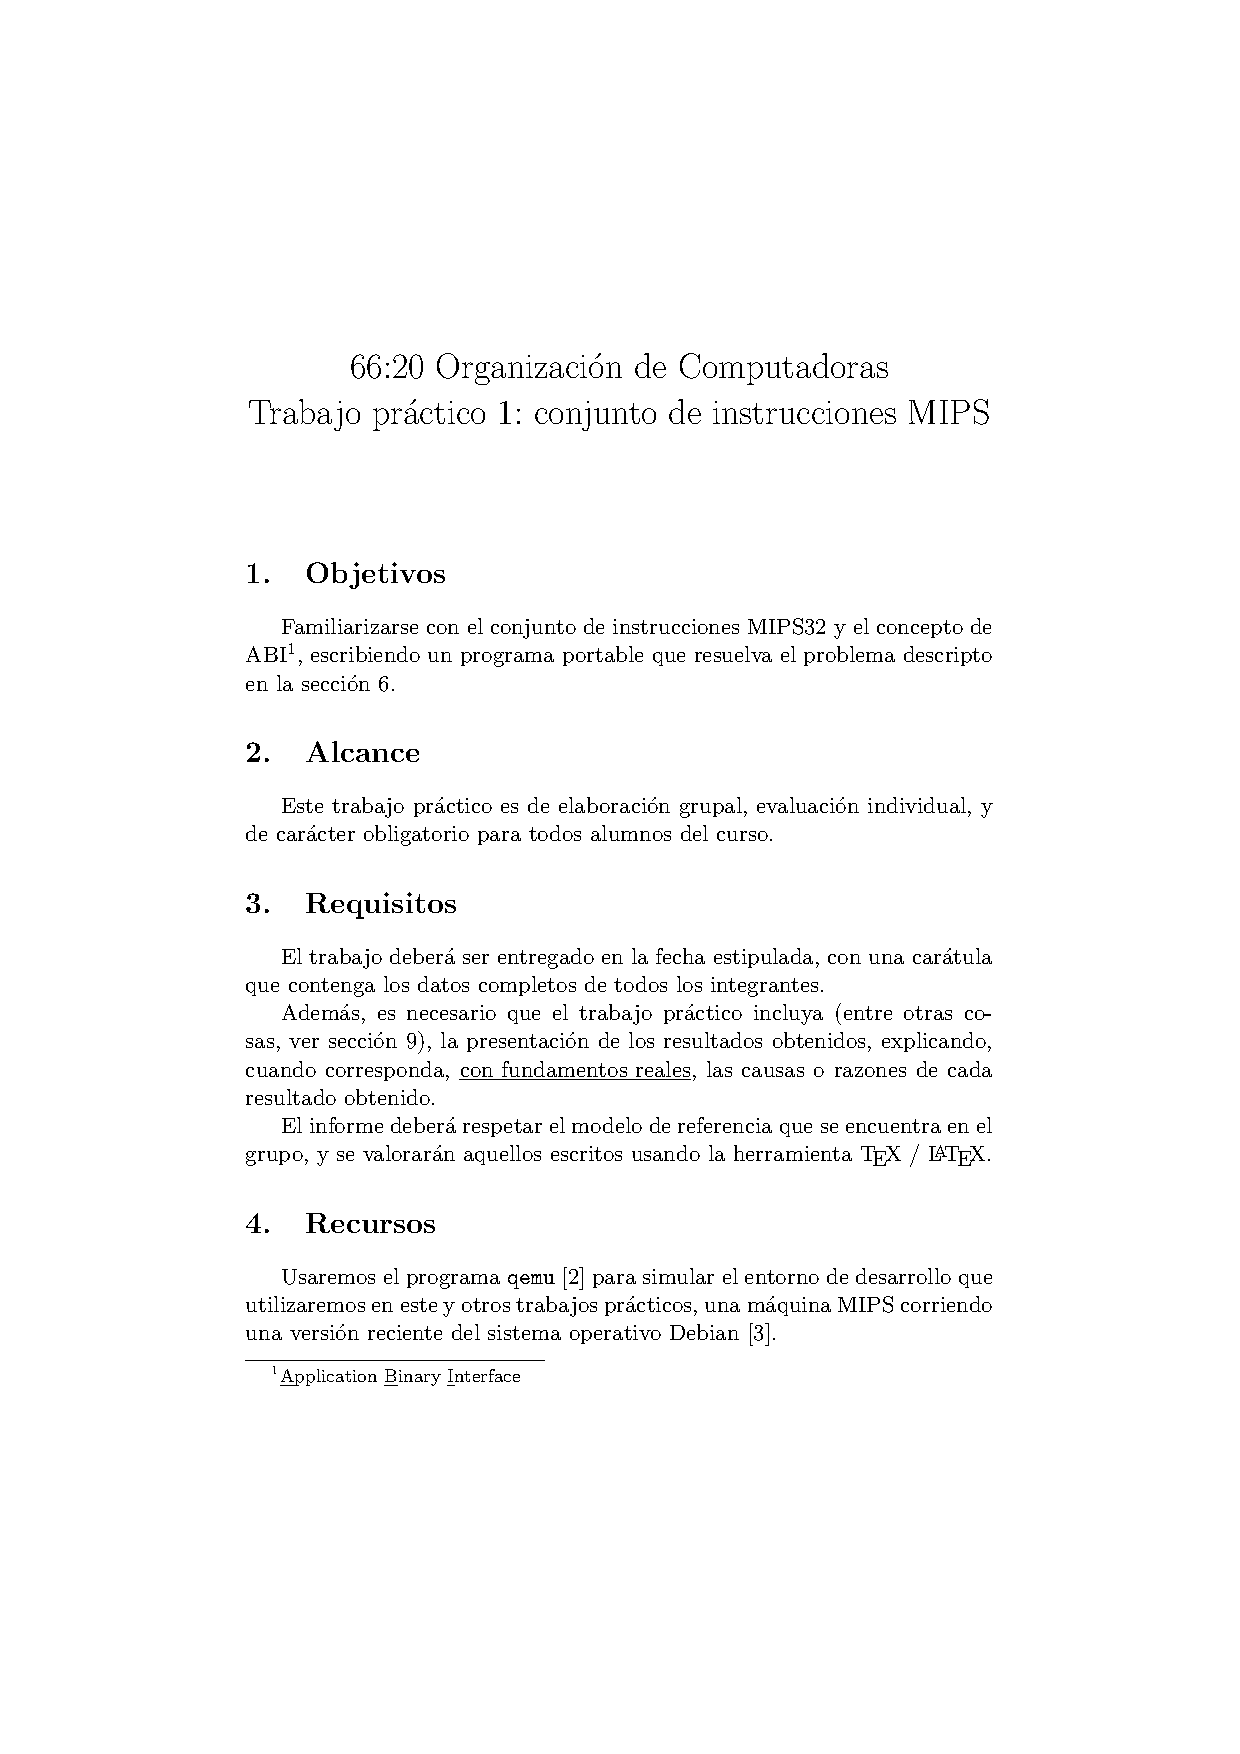
\includepdf[pages=1,scale=0.95,pagecommand = \section{Enunciado del trabajo práctico}\label{enunciado},offset=10 -10]{includes/tp1-c1-2020.pdf}
	\includepdf[pages={2-last},scale=0.95,pagecommand = {},offset=10 -10]{includes/tp1-c1-2020.pdf}
	
	\section{Makefile}\label{appendix_makefile}
	
	\subsubsection{makefile}\label{app_makefile}
	\lstinputlisting[language=bash, style=StyleC]{src/Makefile}
	\clearpage
	
	\section{Tests}\label{appendix_tests}
	
	\subsubsection{run\_tests.sh}\label{app_run_tests}
	\lstinputlisting[language=bash, style=StyleC]{src/run_tests.sh}
	
	\clearpage
	\section{Header files}\label{appendix_headers}
	
	\subsubsection{cmd\_line\_parser.h}\label{app_cmd_line_parser_h}
	\lstinputlisting[language=C, style=StyleC]{src/cmd_line_parser.h}
	\clearpage
	
	\subsubsection{mod.h}\label{app_mod_h}
	\lstinputlisting[language=C, style=StyleC]{src/mod.h}
	\clearpage
	
	\subsubsection{params\_t.h}\label{app_params_t_h}
	\lstinputlisting[language=C, style=StyleC]{src/params_t.h}
	\clearpage
	
	\subsubsection{tablero.h}\label{app_tablero_h}
	\lstinputlisting[language=C, style=StyleC]{src/tablero.h}
	\clearpage
	
	\subsubsection{vecinos.h}\label{app_vecinos_h}
	\lstinputlisting[language=C, style=StyleC]{src/vecinos.h}
	\clearpage
	
	
	\clearpage
	\section{Código fuente}\label{appendix_codigo_fuente}
	
	\subsubsection{cmd\_line\_parser.c}\label{app_cmd_line_parser}
	\lstinputlisting[language=C, style=StyleC]{src/cmd_line_parser.c}
	\clearpage
	
	\subsubsection{conway.c}\label{app_main}
	\lstinputlisting[language=C, style=StyleC]{src/conway.c}
	\clearpage
	
	\subsubsection{mod.c}\label{app_mod}
	\lstinputlisting[language=C, style=StyleC]{src/mod.c}
	\clearpage
	
	\subsubsection{mod.S}\label{app_mod_s}
	\lstinputlisting[language=C, style=StyleC]{src/mod.S}
	\clearpage
	
	\subsubsection{tablero.c}\label{app_tablero}
	\lstinputlisting[language=C, style=StyleC]{src/tablero.c}
	\clearpage
	
	\subsubsection{vecinos.c}\label{app_vecinos}
	\lstinputlisting[language=C, style=StyleC]{src/vecinos.c}
	\clearpage
	
	\subsubsection{vecinos.S}\label{app_vecinos_s}
	\lstinputlisting[language=C, style=StyleC]{src/vecinos.S}
	\clearpage
	
\end{document}
